\chapter{Fundamentação teórica}
\label{CAP2}

Neste capítulo serão abordados os conhecimentos necessários para a compreensão e entendimento sobre Big Data, Hadoop e a importância deles para os dias atuais, serão apresentados conceitos de Big Data, banco de dados, Hadoop e segurança dos dados em Big Data.

\section{Big Data}
\label{BigData}

Big Data é o termo usado para definir grandes volumes de dados. Esses dados são armazenados e processados para que se possam gerar resultados e poder tomar decisões. Governos , Empresas e especialistas utilizam dos dados para prever algumas situações, como por exemplo o Facebook, ele utiliza os dados dos seus usuários para traçar um perfil dele e com isso poder direcionar propagandas de marketing, a Google também consegue fazer isso de acordo com suas pesquisas e seus cliques em sites diversos, a Amazon também possui um sistema de recomendações.

Embora tenha nascido na década de 1990, o termo Big Data começou a ser desenvolvido e utilizado pelo mercado com mais frequência nos últimos anos. Muita gente, entretanto, ainda tem dúvidas sobre o seu real significado, além de sua eficácia e aplicabilidade nos negócios (EXAME, 2013).

\begin{figure}[htbp!] 
	\begin{center}
		% fbox faz uma borda ao redor do seu argumento
		\fbox{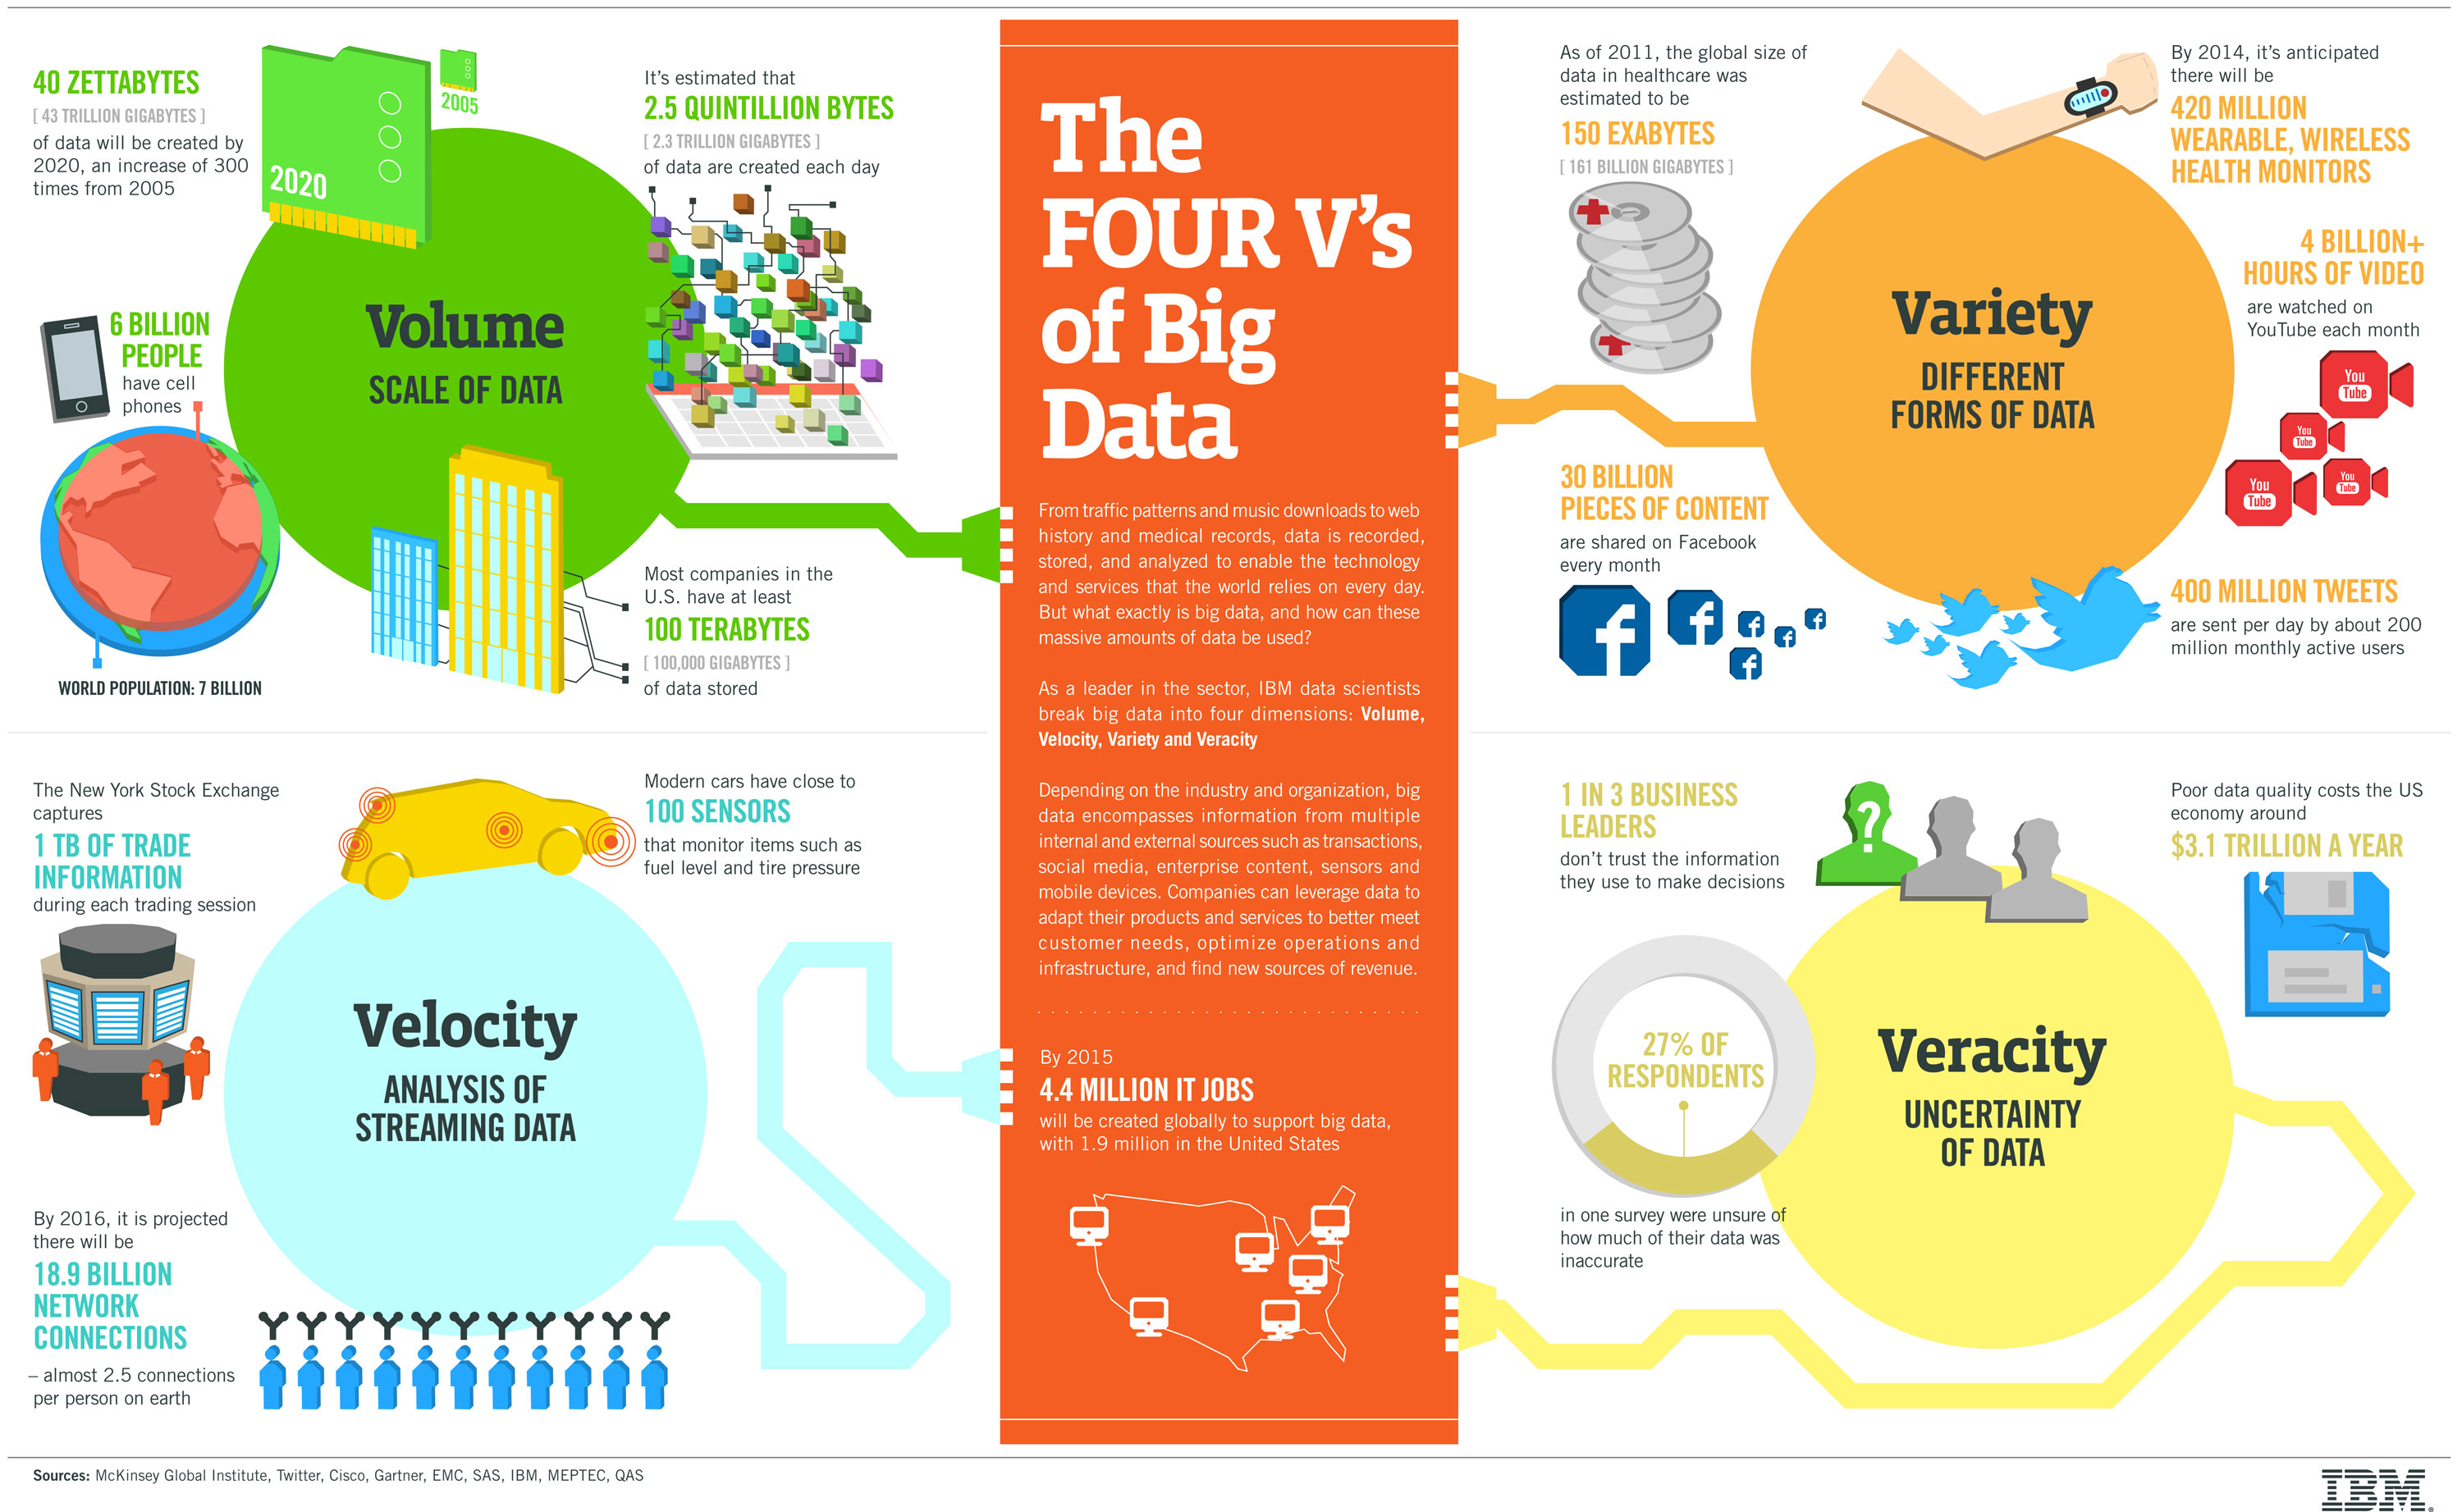
\includegraphics[width=0.80\linewidth]{figures/4-Vs-of-big-data}}
		\caption{Infográfico - The Four V's of Big Data}
		\small{Fonte - (IBM, 2014)}
		\label{Fig:4-Vs-IBM}
	\end{center} 
\end{figure}


A figura \ref{Fig:4-Vs-IBM} mostra que a IBM define Big Data como os 4v's, correspondentes a Volume, Variedade, Velocidade e Veracidade, enquanto que, alguns autores definem o termo Big Data com 5v's, adicionando o termo Valor, porém, isso ainda não é uma unanimidade, tendo em vista que o termo valor é aquilo que se extrai do Big Data, ou o que se espera extrair. Sendo assim, os 4V's são definidos da seguinte forma:

\begin{itemize}

\item \textbf{Volume:} Organizações coletam dados de uma grande variedade de fontes, incluindo transações comerciais, redes sociais e informações de sensores ou dados transmitidos de máquina a máquina.\\

\item \textbf{Velocidade:} Os dados fluem em uma velocidade sem precedentes e devem ser tratados em tempo hábil. Tags de RFID, sensores, celulares e contadores inteligentes estão impulsionando a necessidade de lidar com imensas quantidades de dados em tempo real, ou quase real.\\

\item \textbf{Variedade:} Os dados são gerados em todos os tipos de formatos de dados estruturados, dados numéricos em bancos de dados tradicionais, até documentos de texto não estruturados, e-mail, vídeo, áudio, dados de cotações da bolsa e transações financeiras.\\

\item \textbf{Veracidade:} É a lógica dos dados, necessidade de saber se os dados fazem sentido e saber da sua autenticidade.\\
\end{itemize}
%(SCHONBERGER;CUKIER, 2013, pag. 4)
Para Schonberger e Cukier (2013, pag. 4) "o Big Data se refere a trabalhos em grande escala que não podem ser feitos em escala menor, para extrair novas ideias e criar novas formas de valor de maneiras que alterem os mercados, as organizações, a relação entre cidadão e governos, e entre outros". Tendo em mente o conceito de Big Data, pode-se entender a relação que tem com os bancos de dados da seguinte forma.

\subsection{Banco de dados}

Bancos de dados são os locais que recebem e armazenam os dados. Eles estão em todas as plataformas e serviços, pois os mesmos precisam armazenar informações (TOTALCROSS, 2012). Existem muitos tipos de banco de dados, nos quais podem ser classificados em RDBMS e NoSQL, essa classificação depende de como os dados estão sendo armazenados.

Os bancos de dados relacionais estão organizados em tabelas, onde essas tabelas estão organizadas em forma de linhas e colunas, quando os dados estão sendo armazenados, há uma necessidade de criar o \textit{schema} antes do armazenamento. As relações entre as tabelas ocorrem por meio das chaves primárias e as chaves estrangeiras. Isso difere dos bancos de dados não relacionais, pois o mesmo não existe uma estrutura certa de armazenamento, não há necessidade de criar um \textit{schema} antes, os bancos de dados não relacionais possuem alta performance e escalabilidade, pois todas as informações estão armazenadas em um único registro, onde para acessar as informações são realizadas buscas por chave e valor. Considerando que os bancos de dados não relacionais não possuem uma estrutura definida para armazenar seus dados, eles são ideias para a utilização de Big Data, tendo em vista que o conteúdo de Big Data não tem formato definido.

\subsection{Cluster}

Com a enorme quantidade de dados existentes para serem processados, seria inviável processá-los em uma única máquina, ou seja, existe a necessidade de utilizar o máximo de processadores possíveis para executar essa tarefa em tempo hábil e sem grandes custos. 
	
Com isso surge o chamado cluster, que consiste em uma estrutura computacional formada por várias máquinas, na qual sua função é processar os dados de forma distribuída. 

Existem vários tipos de cluster, cada um com uma funcionalidade ou voltado para uma determinada tarefa, são eles: cluster de alto desempenho, cluster para balanceamento de carga, cluster de alta disponibilidade (INFOWESTER, 2013). Pode ocorrer a combinação de clusters no caso do Hadoop o cluster é utilizado para armazenamento e processamento de dados de forma distribuída.


\section{Apache Hadoop}
\label{Apache Hadoop}

Hoje em dia, graças à internet, a evolução dos sistemas computacionais e a informatização, as grandes empresas criam e armazenam grandes quantidades de dados, porém esses dados precisam ser processados em tempo hábil, para que se possa tomar decisões, pois aquilo que não pode ser medido não pode ser gerenciado (KAPLAN; NORTON, 1997). Se uma empresa conseguir medir seus resultados, conseguir gerenciar seus dados, com certeza sairá na frente das demais e com isso poderá alavancar seus negócios.

O Hadoop é um projeto open-source da Apache Software Foundation que visa proporcionar  computação distribuída, escalável e confiável. Conforme a Apache, o Hadoop é um \textit{framework} que permite o processamento distribuído de grandes conjuntos de dados, por meio de clusters de computadores usando modelos de programação simples, podendo funcionar em um único servidor ou em até milhares de máquinas, cada uma disponibilizando armazenamento e processamento computacional local. Além disso, o Hadoop foi concebido para detectar e tratar falhas na camada de aplicação, fornecendo um serviço altamente disponível sob um conjunto de computadores, todos propensos a falhas (APACHE, 2018).

Considerando o baixo custo, quantidade de dados gerados, a flexibilidade e escalabilidade algumas empresas começaram a utilizar o Hadoop, tais como: Amazon, Facebook, Google, IBM, Intel, Oracle, Yahoo, e entre outras. Tendo em vista que o Hadoop foi projetado para servidores de \textit{hardware} comum, reduzindo os custos dos clusters. O Hadoop é escrito na linguagem de programação java o que permite uma fácil instalação e portabilidade nas máquinas.

Considerando que o Hadoop é um projeto mantido pela Apache Software Foundation, ela também mantém diversos outros projetos que trabalham com armazenamento e processamento distribuído e que podem ser também incluídos no ambiente Hadoop, segundo a definição da própria Apache em sua página \url{hadoop.apache.org}, os outros projetos são definidos da seguinte forma:

\begin{itemize}
\item \textbf{Ambari:} Uma ferramenta baseada na web para provisionamento, gerenciamento e monitoramento de clusters do Apache Hadoop que inclui suporte para Hadoop HDFS, Hadoop MapReduce, Hive, HCatalog, HBase, ZooKeeper, Oozie, Pig e Sqoop. O Ambari também fornece um painel para visualizar a integridade do cluster, como heatmaps e capacidade de visualizar visualmente os aplicativos MapReduce, Pig e Hive, juntamente com recursos para diagnosticar suas características de desempenho de uma maneira amigável ao usuário.

\item \textbf{Avro:} Um sistema de serialização de dados.

\item \textbf{Cassandra:} Um gerenciador de bando de dados escalável, que possui múltiplos nós mestres e portanto não apresenta um ponto de falha único.

\item \textbf{Chukwa:} Um sistema de coleta de dados para gerenciar grandes sistemas distribuídos.

\item \textbf{Hbase:} Um sistema de gerenciador de banco de dados escalável e distribuído, para o armazenamento de Big Data.

\item \textbf{Hive:} Um \textit{software} de data \textit{warehouse} para consultas e gerenciamento de grandes conjuntos de dados armazenados em sistemas de arquivos distribuídos.

\item \textbf{Mahout:} Uma biblioteca escalável para o aprendizado de máquinas e \textit{data mining}.

\item \textbf{Pig:} Uma plataforma para análise de grandes bases de dados, que consiste de uma linguagem de alto nível para expressar programas visando a análise de dados.

\item \textbf{Spark:} Um mecanismos rápido e geral para o processamento de dados em larga escala.

\item \textbf{Tez:} Uma estrutura de programação de fluxo de dados generalizada, criada no Hadoop Yarn, que fornece um mecanismo poderoso e flexível para executar um DAG arbitrário de tarefas para processar dados para casos de uso em lote e interativos. O Tez está sendo adotado pelo Hive, Pig e outras estruturas no ecossistema Hadoop e também por outros \textit{softwares} comerciais para substituir o Hadoop MapReduce como o mecanismo de execução subjacente.

%\nomenclature[ag]{YARN}{Yet Another Resource Negotiator}
%\nomenclature[al]{DAG}{directed acyclic graph}
%\nomenclature[am]{ETL}{Extract Transform Load (Extração Transformação Carregamento)}


\item \textbf{ZooKeeper:} Um serviço centralizado para manter informações de congurações, que proporciona sincronização distribuída e serviços de grupo.
\end{itemize}

O Apache Hadoop é um \textit{framework} para processamento e armazenamento distribuído, isso é realizado graças a os dois principais subprojetos do Apache Hadoop, o Hadoop HDFS e o Hadoop MapReduce, dos quais são explicados a seguir.

\subsection{Hadoop HDFS}

O HDFS — um subprojeto do projeto Apache Hadoop — é um sistema de arquivos altamente tolerante a falhas projetado para executar em \textit{hardware} padrão de baixo custo (HANSON, 2013).
Como sabe, o Apache Hadoop é indicado para armazenamento de grande quantidades de dados, na casa dos pentabytes, e com isso o sistema de arquivos utilizado é o HDFS. O HDFS permite a conexão com os nós, esses nós são os computadores de baixo custo, formando um cluster, onde os dados são distribuídos. 

Segundo o Tom White (2015, pag. 45), o HDFS é um sistema de arquivos distribuído destinado ao armazenamento de grandes arquivos chegando a terabytes com fluxos de acesso a dados padronizados, executado em clusters de servidores comuns. De certo modo, as definições do HDFS, seguem o mesmo padrão, ou seja, é um sistema de arquivo que suporta grandes quantidades de dados e é tolerante a falhas. O HDFS têm muitas similaridades com outros sistemas de arquivos distribuídos, mas é diferente em vários aspectos. Uma diferença notável é o modelo WORM do HDFS que 'afrouxa' as exigências do controle de simultaneidade, simplifica a persistência de dados e habilita acesso de alto rendimento (HANSON, 2013), ou seja, o HDFS é ideal para aplicações que realizam poucas escritas e muitas leituras.%(HANSON, 2013,IBM)
%\nomenclature[af]{WORM:}{write-once-read-many}%

No HDFS, os arquivos são divididos em blocos e replicados em vários nós, e mesmo sendo executado em \textit{hardware} comum e sujeito a falhas de máquinas, o HDFS disponibiliza replicação, detecção de falhas e recuperação de blocos de dados, automaticamente, mantendo a integridade do sistema de arquivos (BRITO, 2014).

\subsubsection{Arquitetura do Hadoop HDFS}

O HDFS segue uma estrutura de mestre e escravo onde o mestre atribui tarefas aos escravos. Os componentes do Hadoop HDFS são:

\begin{itemize}
	\item \textbf{NameNode:}
    Tem como responsabilidade gerenciar os arquivos armazenados no HDFS. Suas funções incluem mapear a localização, realizar a divisão dos arquivos em blocos, encaminhar os blocos aos nós escravos, obter os metadados dos arquivos e controlar a localização de suas réplicas. Como o NameNode é constantemente acessado, por questões de desempenho, ele mantém todas as suas informações em memória. Ele integra o sistema HDFS e fica localizado no nó mestre da aplicação.
	
    \item \textbf{DataNode:}
    Enquanto o NameNode gerencia os blocos de arquivos, são os DataNodes que efetivamente realizam o armazenamento dos dados. Como o HDFS é um sistema de arquivos distribuído, é comum a existência de diversas instâncias do DataNode em uma aplicação Hadoop, para que eles possam distribuir os blocos de arquivos em diversas máquinas. Um DataNode poderá armazenar múltiplos blocos, inclusive de diferentes arquivos. Além de armazenar, eles precisam se reportar constantemente ao NameNode, informando quais blocos estão guardando bem como todas as alterações realizadas localmente nesses blocos.

	\item \textbf{Bloco de arquivos}
    Em geral, os dados do usuário são armazenados nos arquivos da HDFS. O arquivo em um sistema de arquivo será dividido em um ou mais segmentos ou dados armazenados em cada um nós. Esses arquivos são chamados segmentos como blocos. Em outras palavras, o montante mínimo de dados que HDFS pode ler ou escrever é chamado de bloco. O tamanho de bloco padrão é de 64MB, mas pode ser aumentada conforme a necessidade de mudança na configuração HDFS.
    
    \item \textbf{Namespace}
    O HDFS suporta uma organização hierárquica tradicional de arquivos em que um usuário ou um aplicativo pode criar diretórios e armazenar arquivos neles. A hierarquia do namespace do sistema de arquivos é similar à maioria dos outros sistemas de arquivos existentes; é possível criar, renomear, reposicionar e remover arquivos.
    

	\item \textbf{SecondaryNameNode:}
    Utilizado para auxiliar o NameNode a manter seu serviço, e ser uma alternativa de recuperação no caso de uma falha do NameNode. Sua única função é realizar pontos de checagem do NameNode em intervalos pré definidos, de modo a garantir a sua recuperação e atenuar o seu tempo de reinicialização.
\end{itemize}

A figura \ref{Fig:Estrutura HDFS} mostra de maneira geral a estrutura da arquitetura do HDFS e do seu formato de trabalho. 

%link da referencia: https://lakshmana-msbi.blogspot.com.br/2016/01/big-data-hadoop-lesson-5-namenode.html

\begin{figure}[htbp!] \begin{center}
% fbox faz uma borda ao redor do seu argumento
\fbox{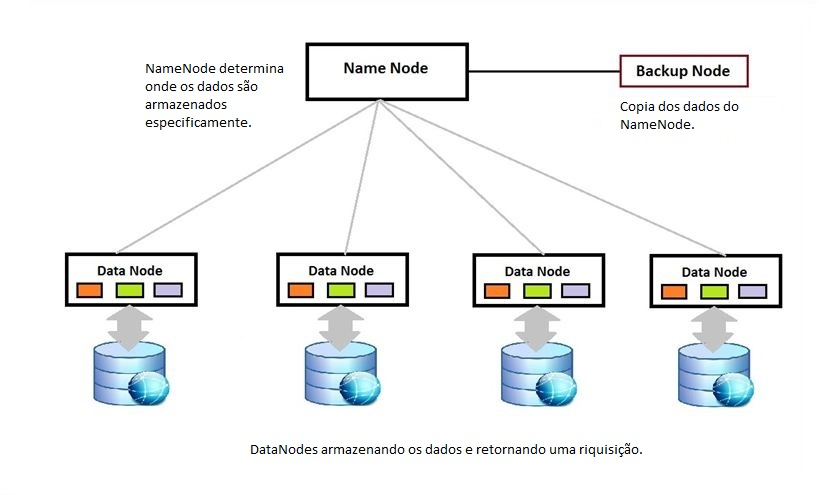
\includegraphics[width=0.80\linewidth]{figures/namenode}}
\caption{Infográfico - Visão geral HDFS }
\small{Fonte - (MSBI, 2016)}
\label{Fig:Estrutura HDFS}
\end{center} \end{figure}


\subsection{Hadoop MapReduce}

MapReduce é um modelo de programação projetado para processamento paralelo e distribuído de grandes conjuntos de dados, criado pela Google, esse paradigma distribui os dados no formato chave-valor, onde a chave é o identificador do registro e valor é o seu conteúdo.

%(LOPES,http://joseguilhermelopes.com.br/hadoop-entenda-arquitetura-hdfs/).

Um trabalho MapReduce normalmente divide o conjunto de dados de entrada em blocos independentes que são processados pelas tarefas do Map de maneira completamente paralela. A estrutura classifica as saídas dos Maps, que são inseridas nas tarefas de \textit{reduce}. Normalmente, tanto a entrada quanto a saída do \textit{Job} são armazenadas em um sistema de arquivos. O \textit{framework} cuida das tarefas de planejamento, monitora-as e re-executa as tarefas com falha (APACHE,2018).

Para Tom White (2015, pag.19 e 22), o MapReduce é um modelo de programação para processamento de dados e que o MapReduce funciona dividindo o processo em duas partes, ou seja, na fase Map e na fase \textit{Reduce}.

O MapReduce consegue abstrair a programação paralela em apenas duas funções, a Map e a \textit{Reduce} facilitando a vida do desenvolvedor, como demonstra a figura \ref{Fig:Estrutura Mapreduce01}.

\begin{figure}[htbp!] \begin{center}
% fbox faz uma borda ao redor do seu argumento
\fbox{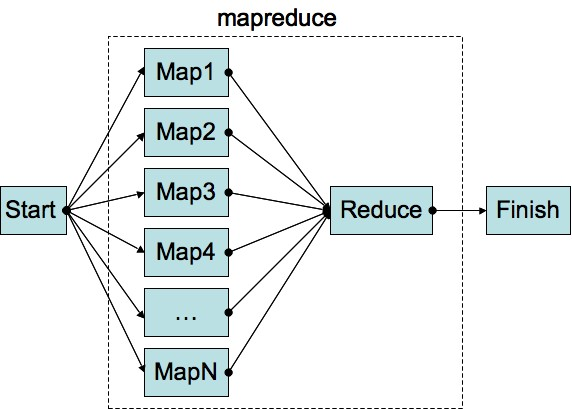
\includegraphics[width=0.60\linewidth]{figures/mapreduce}}
\caption{Infográfico - Visão geral do funcionamento do MapReduce }
\small{Fonte - (LOPES, 2016)}
\label{Fig:Estrutura Mapreduce01}
\end{center} \end{figure}


\subsubsection{arquitetura do MapReduce}

Como pode-se observar na figura \ref{Fig:Estrutura MapReduce02}, a arquitetura MapReduce é semelhante a arquitetura do HDFS, sendo também baseada em mestre e escravo, onde o JobTracker é o mestre e o TaskTracker é o escravo. Segundo Tom White (2015, pag. 83) esses dois componentes do MapReduce são definidos da seguinte forma:


\begin{figure}[htbp!] \begin{center}
% fbox faz uma borda ao redor do seu argumento
\fbox{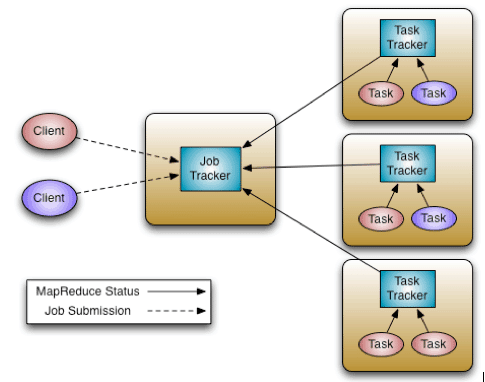
\includegraphics[width=0.80 \linewidth]{figures/mapReduce}}
\caption{Infográfico - Visão geral MapReduce }
\small{Fonte - (HORTONWORKS, 2012)}
\label{Fig:Estrutura MapReduce02}
\end{center} \end{figure}
%link da figura: 
%https://br.hortonworks.com/blog/apache-hadoop-yarn-background-and-an-overview/


\begin{itemize}
	\item \textbf{JobTracker:} Assim como o NameNode, o JobTracker também possui uma função de gerenciamento, porém, nesse caso, o controle é realizado sobre o plano de execução das tarefas a serem processadas pelo MapReduce. Sua função é designar diferentes nós para processar as tarefas de uma aplicação e monitorá-las enquanto estiverem em execução. Um dos objetivos do monitoramento é, em caso de falha, identificar e reiniciar uma tarefa no mesmo nó ou, em caso de necessidade, em um nó diferente.\\
    
    \item \textbf{TaskTracker:} Processo responsável pela execução de tarefas MapReduce. Assim como os DataNodes, uma aplicação Hadoop é composta por diversas instâncias de TaskTrackers, cada uma em um nó escravo. Um TaskTracker executa uma tarefa Map ou uma tarefa \textit{Reduce} designada a ele. Como os TaskTrackers rodam sobre máquinas virtuais, é possível criar várias máquinas virtuais em uma mesma máquina física, de forma a explorar melhor os recursos computacionais.
\end{itemize}

Apesar da solução Hadoop com HDFS e o MapReduce ser muito útil para diversas aplicações, foram encontradas algumas limitações em sua versão 1.0, segundo Tom White (2015, pag.84), o MapReduce tinha uma limitação quando se trabalhava com cerca de 4000 mil nós e 40000 mil tarefas, pois o JobTracker ficava sobrecarregado e com isso era gerado uma perda de performance em cascata, outro problema encontrado era quando o JobTracker falhasse, todo restante da aplicação, ou seja, os taskTracker também falhavam, e tudo era perdido, com isso houve a necessidade de uma atualização, dai surgiu o Yarn, o Hadoop foi atualizado para a versão 2.0 e junto com ele vem o \textit{framework} Yarn onde será explicado na próxima seção.

\subsection{Apache Hadoop YARN}

Como explicado anteriormente, o MapReduce na versão 1.0 sobrecarregava muito o JobTracker, com isso ocasionava uma falha em cascata, pois o JobTracker tinha o papel de gerenciar, monitorar e verificar falhas, sendo assim surge o \textit{Framework} Yarn, também é um \textit{framework} para trabalhar com processamento e armazenamento distribuído. O Yarn é um gerenciador de aplicativos distribuídos e de uso geral que veio pra substituir a antiga estrutura do MapReduce na qual se concentravam as taferas e o gerenciamento apenas no JobTracker. Com o Yarn, o gerenciamento que antes era realizado pelo JobTracker agora passa a ser gerenciado pelo Yarn, onde o mesmo possui uma estrutura diferenciada para tal atividade. O Yarn possui os componentes ResourceManager, NodeManager e o ApplicationMaster, todos irão executar as tarefas que antes eram executadas apenas pelo JobTracker. Segundo a Hontonworks, os componentes do Yarn são definidos da seguinte forma:




\begin{comment}
\begin{figure}[htbp!] \begin{center}
% fbox faz uma borda ao redor do seu argumento
\fbox{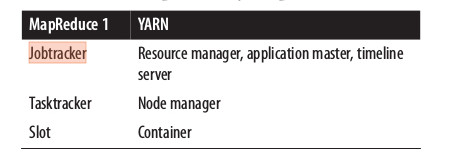
\includegraphics[width=0.80\linewidth]{figures/comparacaoYarn_mapReduce01}}
\caption{Comparação - Yarn e MapReduce 1}
\small{Fonte - (WHITE, 2015)}
\label{Fig:Comparação - Yarn e MapReduce 1}
\end{center} \end{figure}
\end{comment}



\begin{itemize}

\item \textbf{ResourceManager:}
Possui um escalonador conectável, que é responsável por alocar recursos para vários aplicativos em execução, sujeitos a restrições familiares de capacidades, filas, e entre outras. O Agendador é um agendador puro no sentido de que não realiza monitoramento ou rastreamento de status para o aplicativo, não oferecendo garantias sobre a reinicialização de tarefas com falha devido a falhas de aplicativos ou falhas de \textit{hardware}. O Agendador executa sua função de agendamento com base nos requisitos de recursos dos aplicativos; Ele faz isso com base na noção abstrata de um recipiente de recursos que incorpora elementos de recursos como memória, CPU, disco, rede, e entre outros.

\item \textbf{NodeManager:}
É o escravo por máquina, que é responsável por lançar os recipientes dos aplicativos, monitorar o uso de recursos e relatar o mesmo ao ResourceManager.

\item \textbf{ApplicationMaster:}
Tem a responsabilidade de negociar contêineres de recursos apropriados do \textit{Scheduler}, rastreando seu status e monitorando o progresso. Da perspectiva do sistema, o próprio ApplicationMaster é executado como um contêiner normal.

\end{itemize}

Como ilustra a figura \ref{Fig:Estrutura YARN}, após instalado o Yarn, tem-se uma arquitetura similar ao MapReduce versão 1.0, porém com algumas vantagens, sendo uma delas de que se o nó mestre parar de funcionar toda a aplicação ainda continua funcionando, coisa que não acontecia na versão 1.0 do Hadoop.


\begin{figure}[htbp!] \begin{center}
% fbox faz uma borda ao redor do seu argumento
\fbox{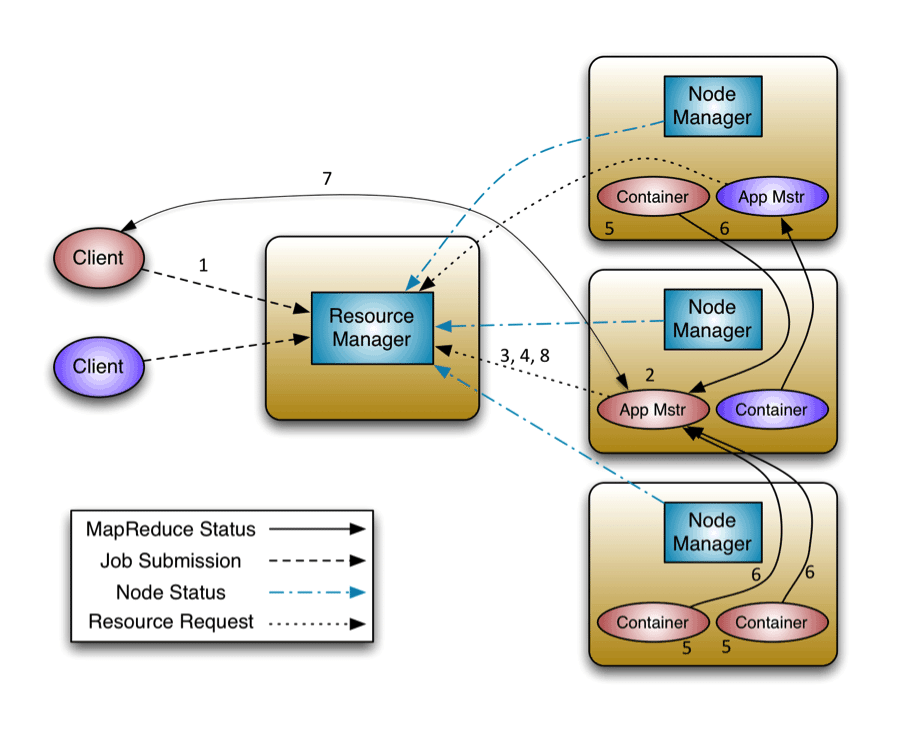
\includegraphics[width=0.80\linewidth]{figures/yarnflow}}
\caption{Infográfico - Visão geral YARN }
\small{Fonte - (Apache, 2018)}
\label{Fig:Estrutura YARN}
\end{center} \end{figure}

\newpage
\subsection{Segurança do Hadoop}

Nas versões anteriores do Hadoop a segurança fornecida é a que o cluster será utilizado por um grupo de usuários fechado, e as medidas de segurança são para evitar perdas acidentais e não autenticação (WHITE, 2015).

Com a replicação dos dados em nós diferentes, isso faz com que em casos de perda de dados, ou por descuido de algum usuário, os dados possam ser recuperados, pois existem cópias deles em outros nós. Isso não impede que usuário possa entrar como root e excluir todos os arquivos da raiz.

O que faltava para o Hadoop era um mecanismo de autenticação que garantisse que aquele usuário que estava tentando realizar tal atividade era ele mesmo (WHITE, 2015). A segurança do Hadoop é a autorização, apenas identifica se o usuário tem ou não a permissão para executar aquela tarefa desejada.

De acordo com White (2015) a autorização não é suficiente por si só, porque o sistema ainda está aberto ao abuso por meio de falsificação por um usuário mal-intencionado que pode ganhar rede e acesso ao cluster.

A instalação do Apache Hadoop não traz consigo uma segurança baseada em autenticação, com isso, faz necessário a implementação do protocolo kerberos.

\subsubsection{Protocolo Kerberos}

O Kerberos foi criado em meados dos anos 80, no instituto de tecnologia de Massachusetts, por Clifford Neuman e Steve Miller, ele foi desenvolvido durante durante o Projeto Athena, usando como base o protocolo Needham-Schroeder (LUZ, 2011).
%https://www.profissionaisti.com.br/2011/11/conhecendo-o-protocolo-de-rede-kerberos/
A ideia principal do protocolo é evitar a entrada de usuários estranhos na rede, ou seja, só entra usuários autenticados, e a autenticação do protocolo funciona por três serviços, três servidores. 
%https://www.gta.ufrj.br/grad/02_2/kerberos/

\begin{itemize}

\item \textbf{Servidor de Autenticação (SA):} Responsável pela autenticação em si do usuário, pois a partir de um pedido a este servidor, ele receberá um ticket e uma chave de sessão, podendo assim continuar tentando se conectar com o sistema.\\

\item \textbf{Servidor de Concessão de Ticket (TGS):} É o responsável pela concessão dos tickets para os serviços que utilizam o Kerberos.\\

\item \textbf{Servidor de Administração (KADM):} Responsável pelo controle das chaves secretas, cadastrando-as tanto no cliente quanto no servidor. Para isso o usuário precisa fazer o seu cadastramento, escolhendo um username e uma senha.\\

\end{itemize}

\begin{figure}[htbp!] 
\begin{center}
% fbox faz uma borda ao redor do seu argumento
\fbox{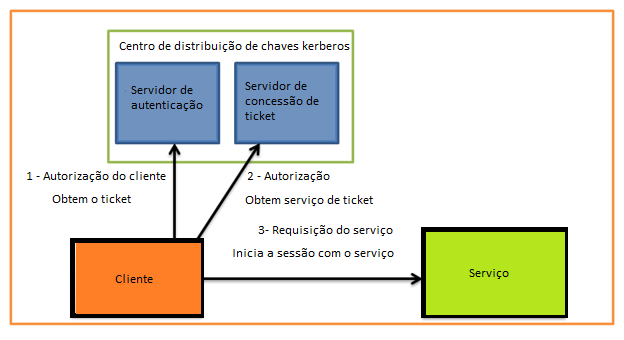
\includegraphics[width=0.80\linewidth]{figures/funcionamentoKerberos}}
\caption{Visão do funcionamento do kerberos }
\small{Fonte - (DROIDHUB, 2014)}
\label{Fig:Visão do funcionamento do kerberos}
\end{center} 
\end{figure}

O funcionamento do kerberos possui muitas vantagens, uma delas é que as senhas duram poucas horas, ao realizar uma requisição ao servidor de autenticação e depois ao servidor de concessão de ticket o usuário garente uma senha, porém ela dura por no máximo 8 horas, dificultando assim alguma tentativa de força bruta. 

Muitas aplicações podem ser protegidas pelo kerberos, tais como: ssh, telnet, linux, e entre outros. A figura \ref{Fig:Visão do funcionamento do kerberos} ilustra uma visão geral do funcionamento do protocolo kerberos, demonstrando que antes de tudo o cliente faz uma requisição para os servidores kerberos e logo após isso é que terá acesso ao servidor, que pode ser um ambiente Hadoop.

\section{Tipos de ataques à segurança}

Nos dias de hoje existem milhares de ataques diferentes, porém, neste trabalho foram utilizados três dos mais conhecidos no mundo da segurança da informação, eles são simples na sua forma de execução, mas o resultado pode ser desastroso para a vítima, sendo assim, são eles:
%\nomenclature[da]{DOS:}{Denial Of Service}%

\begin{itemize}
\item \textbf{DoS:} É uma tentativa de fazer com que aconteça uma sobrecarga em um servidor ou computador comum para que recursos do sistema fiquem indisponíveis para seus utilizadores (CANALTECH, 2018). Essa prática de ataque não tem a intenção de invadir o sistema, mas tem a pretensão de deixar o sistema indisponível para os usuários, enviando muitos pacotes de requisições, na qual irá sobrecarregar a vítima, pois ela não irá conseguir responder todas as requisições e com isso irá ficar indiponível.\\
%https://canaltech.com.br/produtos/O-que-e-DoS-e-DDoS/

Ataques DDoS são executados há tempos e já prejudicaram empresas bastante conhecidas. Historicamente, servidores da CNN, Amazon, Yahoo, Microsoft e eBay já foram "vítimas". Em dezembro de 2010, por exemplo, os sites da Visa, Mastercard e Paypal sofreram ataques DDoS de um grupo defendendo a não existência de "censura" na internet. Em fevereiro de 2012, ataques foram executados contra sites de bancos brasileiros por motivos semelhantes (ALECRIM, 2012).\\
%https://www.infowester.com/ddos.php

\begin{figure}[htbp!] 
\begin{center}
% fbox faz uma borda ao redor do seu argumento
\fbox{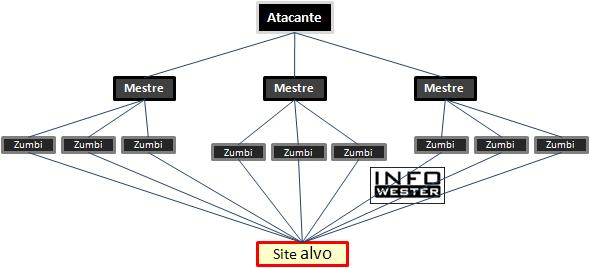
\includegraphics[width=0.80\linewidth]{figures/ddos}}
\caption{Visão do funcionamento de um DDoS}
\small{Fonte - (INFOWESTER, 2012)}
\label{Fig:Visão do funcionamento de um DDOS}
\end{center} 
\end{figure}

A figura \ref{Fig:Visão do funcionamento de um DDOS} mostra uma visão geral do funcionamento de um DDoS, o ataque de negação de serviço utilizado neste trabalho consiste em apenas uma máquina enviando pacotes para outra máquina, na tentativa de sobrecarregar o serviço e assim poder visualizar seu comportamento mediante ataques.\\

\item \textbf{Metasploit framework: } Plataforma de teste de penetração modular baseada em Ruby que permite escrever, testar e executar código de exploração. O \textit{Metasploit Framework} contém um conjunto de ferramentas que pode ser usada para testar vulnerabilidades de segurança, enumerar redes, executar ataques e evitar a detecção. Em sua essência, o \textit{Metasploit Framework} é uma coleção de ferramentas comumente usadas que fornecem um ambiente completo para testes de penetração e desenvolvimento de exploração.\\
%https://metasploit.help.rapid7.com/docs/msf-overview

Esse \textit{framework} possui um conjunto de ferramentas que podem ser acessadas pelo seu console msf. Nesta aplicação foi utilizado uma das suas ferramentas de força bruta, que pode ser utilizado nos seguintes protocolos: ssh, telnet e ftp. Essa ferramenta é formada por um conjunto de \textit{exploit}, que podem encontrar vulnerabilidades diversas nos sistemas.\\

\item \textbf{Man in the middle: } Traduzindo do inglês para o português como homem no meio, significa que o atacante irá ficar entre dois terminais, ou seja, no meio da conexão entre as duas vítimas, interceptando todo tráfego de comunicação entre essas duas máquinas. Esse ataque pode ter algumas variantes, através dele pode-se clonar o browser das vítimas, enviar e-mails falsos, e entre outros. Esse ataque é muito difícil de detectar, pois ambos os usuários pensam que estão se comunicando sem que ninguém perceba. Neste trabalho foi utilizado esse ataque e com a ferramenta ettercap, foi possível conseguir poluir a tabela ARP de um host, com isso, foi possível saber que ele estava se reportando para a máquina atacante, ao invés de se reportar para a máquina verdadeira, como ilustrado na figura \ref{Fig:Visão geral do mitm}.
%http://www.webcheats.com.br/threads/6-ataque-man-in-the-middle.2552630/
%\nomenclature[db]{MITM:}{Man in the middle}%


%ajeitar a legenda
\begin{figure}[htbp!] 
\begin{center}
% fbox faz uma borda ao redor do seu argumento
\fbox{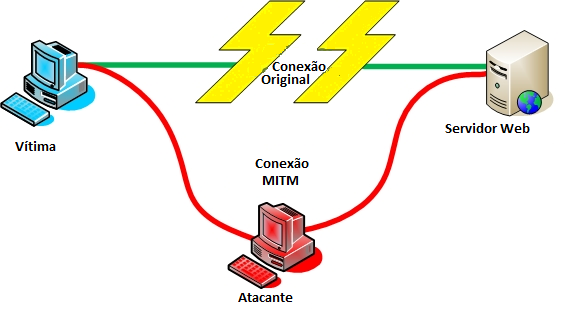
\includegraphics[width=0.80\linewidth]{figures/manInTheMiddle}}
\caption{Visão geral de um MITM }
\small{Fonte - (DARKMOREOPS, 2016)}
\label{Fig:Visão geral do mitm}
\end{center} 
\end{figure}

\item \textbf{Protocolo ARP: } O protocolo ARP é o mecanismo responsável pela associação do endereço MAC a um endereço IP, da seguinte forma: Se um hostA pretende se comunicar com um hostB, então o hostA pega o endereço IP do hostB e envia pra rede em broadcast "peguntando quem tem o endereço físico correspondente aquele IP", com isso, o hostB "responde com o endereço físico, ou seja, o endereço MAC". Dai o hostA guarda em uma tabela, a tabela ARP, o endereço IP e o endereço MAC correspondentes, e com isso pode ocorrer a comunicação (PINTO, 2011).

%\nomenclature[dc]{ARP:}{Address Resolution Protocol}%
%\nomenclature[dd]{IP:}{Internet Protocol}%
%\nomenclature[de]{MAC:}{Media Access Control}%
%https://pplware.sapo.pt/microsoft/windows/redes-sabe-para-que-serve-o-protocolo-arp/
\end{itemize}

%\newpage
\section{PenTest}

O \textit{PenTest}, também conhecido como Teste de Intrusão, é um teste realizado em uma rede ou um sistema de computadores com o objetivo de descobrir vulnerabilidades no sistema. Através desse teste um Pentester pode descobrir todas as vulnerabilidades encontradas em uma rede e até mesmo descobrir qual o tamanho do dano que uma invasão causaria aos computadores e a rede.

Existem dois tipos de \textit{PenTest}, o \textit{Blackbox} e \textit{Whitebox}, cada tipo de teste é feito para descobrir diferentes problemas e para prever diferentes tipos de ataques.

\subsubsection{Whitebox}
O \textit{Whitebox} é um teste realizado com o Pentester sabendo todas as informações sobre a rede como topografia, IPs, senhas, níveis de usuários e logins. Esse é o mais amplo de todos os testes e é capaz de encontrar qualquer vulnerabilidade.

\subsubsection{Blackbox}
O \textit{Blackbox} é um teste mais voltado para situações reais onde o testador não terá nenhuma informação sobre o sistema, quase como um teste cego.

Esse teste é muito próximo do que acontece na vida real quando um \textit{cracker} tenta quebrar a segurança de uma rede e é atualmente o mais requisitado pelas empresas. %( http://ninjadolinux.com.br/o-que-e-pentest/  ); (Cassio Augusto Fevereiro 10, 2017 )

\subsection{Fases de um PenTest}
Uma análise de \textit{PenTest} consiste em fases bem definidas e organizadas, normalmente divididas em um ciclo de vida, na qual cada fase possui diferentes etapas, definidas a seguir.

\subsubsection{Fase de Reconhecimento}
Nessa fase a equipe de PenTesters realiza o levantamento do máximo de informações possíveis sobre a empresa analisada. Dados como os serviços prestados, os principais gerentes e diretores, localização física, existência de filias, e entre outras.

\subsubsection{Fase de Varredura}
Nesse momento é realizado uma varredura do que está presente na rede. Por exemplo, o range de IPs que é utilizado, quais os servidores existentes, os sitemas operacionais utilizados, as portas abertas, e entre outras.

\subsubsection{Fase de Obtenção de Acesso e Exploração}
Com base no que foi identificado na fase de varredura, o PenTester fará a exploração de cada item, efetivamente em busca das vulnerabilidades existentes. Com o uso de técnicas de \textit{exploit} e \textit{brute force} tentará identificar quais serviços estão vulneráveis e que tipo de informação, falhas ou controles podem ser obtidos através daquele serviço.

\subsubsection{Fase de Obtenção de Evidências e Reporte}
As evidências de todas as falhas e vulnerabilidades identificadas são coletada pela equipe. Com base nessas informações, é gerado um relatório completo indicando os pontos vulneráveis de todos os elementos da empresa, falhas na rede, em \textit{software} mal configurados e desatualizados, falta de elementos de segurança, e entre outros, indicando inclusive que prejuízos podem ser causados à empresa em cada uma das falhas.
%(http://profissaohacker.com/pentest/);
%(AJEITAR ISSO AQUI)

Para realizar os teste de invasão os Pentesters utilizam diversas ferramentas e sistemas operacionais, mas o sistema mais utilizado é o kali linux, definido a seguir.

\subsection{Kali Linux}
	Uma das ferramentas mais indicadas pelos profissionais da área de segurança da informação é o Kali Linux (antigo Backtrack) que é um sistema operacional feito para \textit{hackers} e para a realização de testes de intrusão. O Kali é uma distribuição Linux, baseada em Debian que possui centenas de ferramentas para realização de testes de segurança e para exploração de vulnerabilidades (AUGUSTO, 2017).
    De acordo com a página oficial do kali linux, na sua documentação ele é definido como

\begin{flushright}
\small\it
	"O Kali Linux é uma distribuição Linux baseada no Debian destinada a testes avançados de penetração e auditoria de segurança. Kali contém várias centenas de ferramentas que são voltadas para várias tarefas de segurança da informação, tais como, testes de penetração, pesquisa de segurança, computação forense e engenharia reversa. O Kali Linux é desenvolvido, financiado e mantido pela Offensive Security, uma empresa líder em treinamento de segurança da informação" (KALI LINUX, 2018).
\end{flushright}

Além disso, ainda de acordo com a pagina oficial, o kali linux possui mais de 600 ferramentas de teste de penetração, é livre de código aberto e possui diversos suportes, tornando-se assim a ferramenta ideal e preferida para profissionais da área de segurança da informação.

%https://www.kali.org/
%(09/05/2018)

Com as ferramentas que o kali linux oferece é possivel realizar diversos tipos de testes de penetração, seguindo a ordem de um ataque que é desde o levantamento de informações até a obtenção dos dados, em cada fase dos ataques existem um conjunto de ferramentas designadas.

Dentre todas as ferramentas existentes no sistema operacional kali linux, existem algumas que merecem destaque e que são quase sempre utilizadas para realizar algum tipo de ataque, são elas:

\begin{itemize}
\item \textbf{Nmap:} A página oficial do nmap o define como
\begin{flushright}
\small \it
	"O Nmap é uma ferramenta de código aberto para exploração de rede e auditoria de segurança. Ela foi desenhada para escanear rapidamente redes amplas, embora também funcione muito bem contra hosts individuais" (NMAP, 2018).\\
\end{flushright}
%(https://nmap.org/man/ptBR/index.html) (09/05/2018)\\

\item \textbf{Wireshark:} O Wireshark é um analisador de protocolos de rede, ele analisa o tráfego da rede de forma minunciosa.\\

\item \textbf{Metasploit framework:} Esse \textit{framework} consiste de um conjunto de aplicações que são utilizadas para testes de invasão.\\

\item \textbf{Ettercap:} Mais uma ferramenta para testes de invasão, ela é muito utilizada para realizar ataque \textit{man in the middle}, ou seja, homem no meio traduzindo para o português.

\item \textbf{Aircrack-ng:} Essa ferramenta é utilizada para quebrar senhas de redes wireless.
\end{itemize}

Essas são apenas algumas das poderosas ferramentas que o kali linux tem a sua disposição, considerando que o sistema é de código aberto, cada profissional pode ter sua ferramenta customizada. Em ataques \textit{hacker} quase sempre são utilizadas as ferramentas citadas acima, pois cada uma tem um propósito específico e juntas formam um combinado de técnicas que auxiliam o PenTester em suas análises.


%A Figura \ref{Fig:1} mostra o exemplo do uso do comando ``subfigure''. Apesar de aceitar diferentes tipos de imagens. É preferível que as imagens estejam no formato .eps. Isso garante que a imagem impressa seja exatamente aquela visualizada, como acontece com arquivos pdf.

%\begin{figure}[!ht]
%\centering
%\subfloat[]{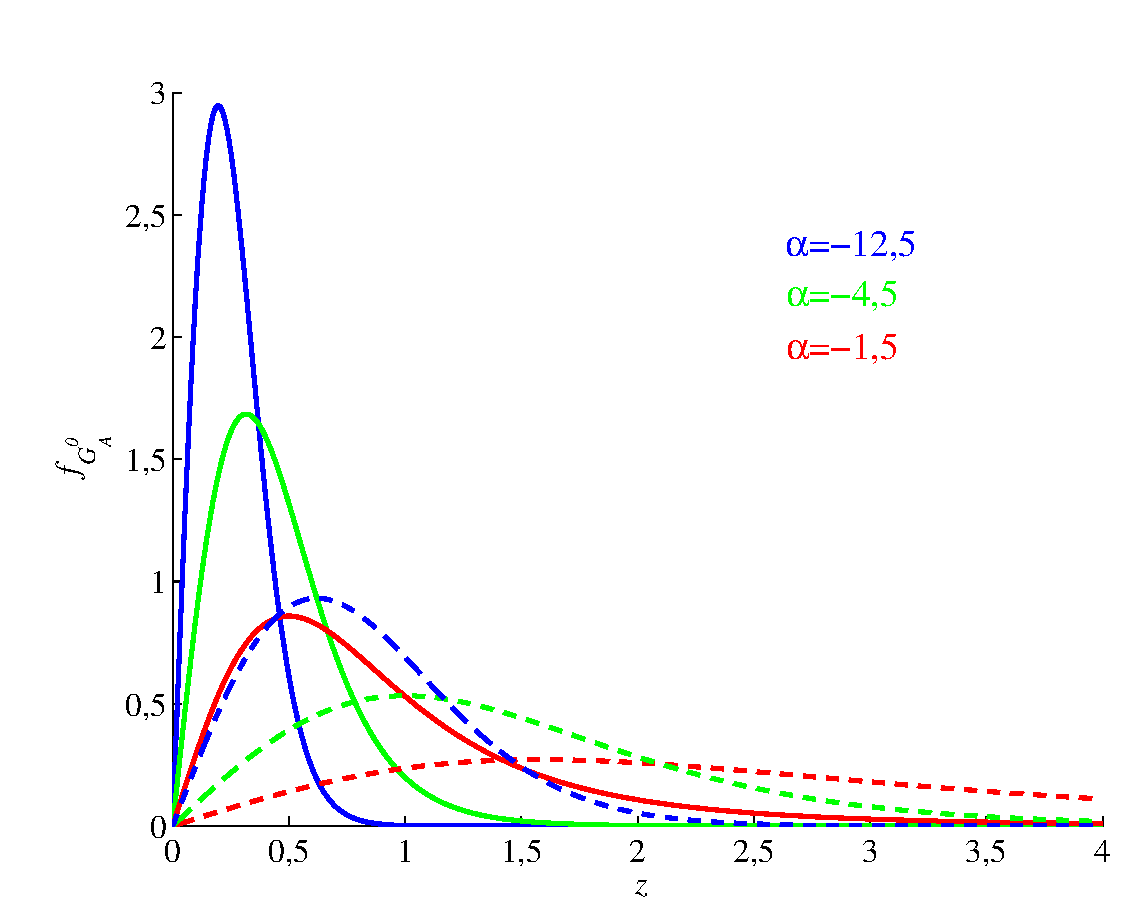
\includegraphics[scale=.65]{figures/fig1.eps}}\\
%\subfloat[]{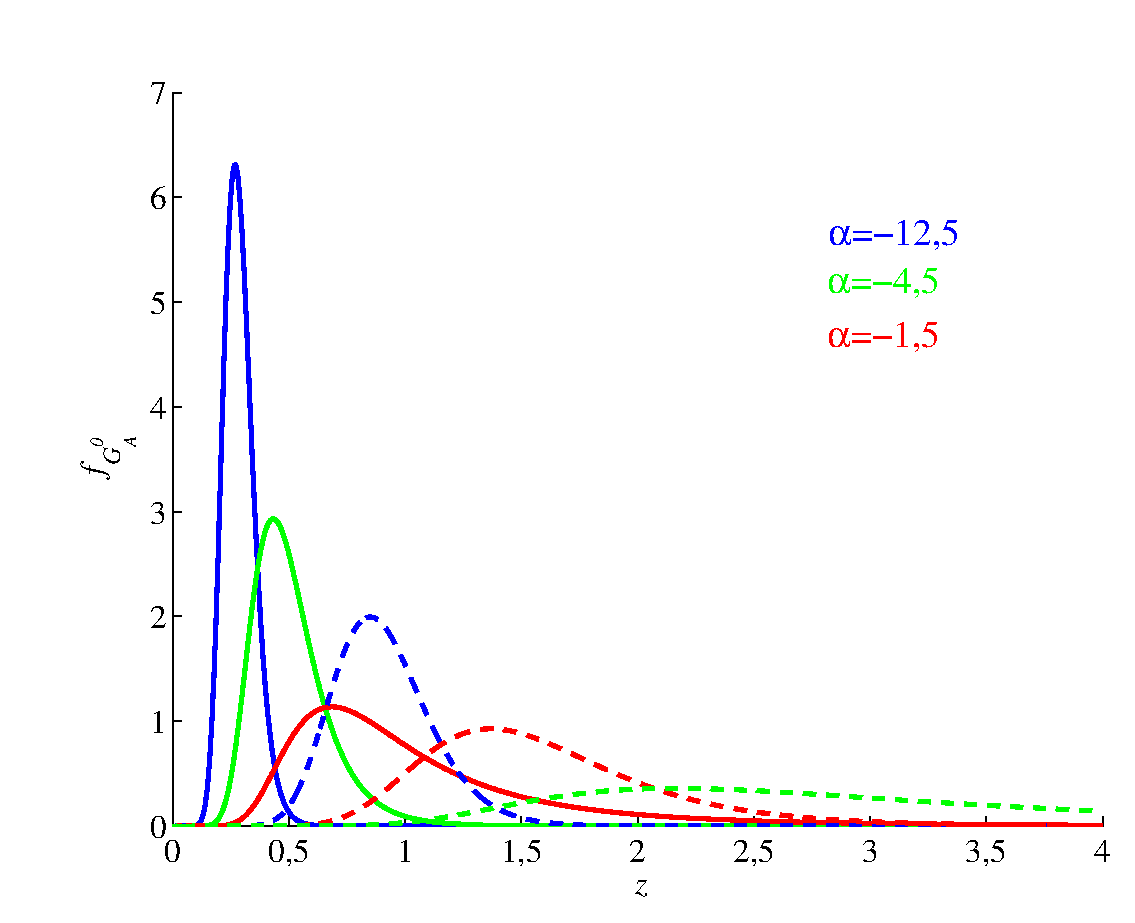
\includegraphics[scale=.65]{figures/fig2.eps}}
%\caption{ Curvas de funções de probabilidade: (a) exemplo 1, (b) exemplo 2.} \label{Fig:1}
%\end{figure}